%%%%%%%%%%%%%%%%%%%%%%%%%%%%%%%%%%%%%%%%%%%%%%%%
% Author: Damodar Rajbhandari                  %
% Created on: 08:45 pm, July 11,Tuesday, 2017  %
% Updated on: 10:30 pm, July 11,Tuesday, 2017  %
% License: GNU General Public License v3.0     %
%%%%%%%%%%%%%%%%%%%%%%%%%%%%%%%%%%%%%%%%%%%%%%%%

\documentclass[a4paper,10pt]{article}

\usepackage[utf8]{inputenc}
\usepackage{graphicx}
\graphicspath{{images/}{../images/}}

\usepackage{geometry}
\geometry{left = 1.7cm, right= 1.7cm}

\usepackage{fancyhdr}
\usepackage{url}


\pagestyle{fancy}
\fancyhf{}

\lhead{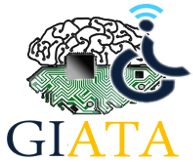
\includegraphics[width=2.3cm, height= 1.73cm]{Logo-GIIATa-small.png}}

\chead{{\itshape \bfseries \textquotedblleft Taller de Visión por Computador: \\fundamentos y experiencias para proyectos humanitarios\textquotedblright} \\
{\bfseries GI-IATa, Cátedra UNESCO Tecnologías de apoyo\\para la Inclusión Educativa}\\
Universidad Politécnica Salesiana, Sede Cuenca}

\rhead{
\includegraphics[width=3.33cm, height= 1.5cm]{logo-catedra.png}}
\renewcommand{\headrulewidth}{1.5pt}

\usepackage{hyperref}

\begin{document}
\vspace*{2.1cm}

\begin{center}
\bfseries \LARGE Especificaciones del proyecto final
\end{center}

\vspace{0.1cm} 

\section{Objetivo general}

El taller de visión por computador con enfoque en proyectos humanitarios busca despertar el interés en el desarrollo de aplicaciones que permitan contribuir en la creación de tecnologías de inclusión educativa y asistencia de poblaciones vulnerables\footnote{Este documento se ha desarrollado empleando \LaTeX~ y en base al código creado por Damodar Rajbhandari: \url{https://github.com/vlarobbyk/LaTeX}}.

Este taller está dirigido a estudiantes de diferentes carreras de la Universidad Politécnica Salesiana, Sede Cuenca que no solo buscan mejorar sus conocimiento, sino también ayudar a cimentar una sólida base tecnológica con visión solidaria.


\section{Objetivos específicos}

\begin{itemize}
	\item Consolidar los conocimientos que se adquirieron durante las clases desarrolladas en el taller.
	\item Implementar una aplicación que emplee técnicas de visión artificial como detección y/o reconocimiento facial, aplicaciones de visión artificial para dispositivos embebidos Raspberry PI, control de actuadores y fundamentos de visión en robótica básica.
	\item Familiarizarse con los fundamentos del desarrollo de aplicaciones de visión artificial para contribuir en la solución de problemas sociales.
\end{itemize}


\section{Visión por computador aplicada a proyectos humanitarios}

Hoy en día existen diversas aplicaciones que emplean técnicas de visión artificial con el fin de brindar soporte en diferentes ámbitos del cuidado de la salud, la inclusión educativa y la investigación en general.

A continuación presentaremos algunos de los proyectos que se han desarrollado dentro del Grupo de Investigación en Inteligencia Artificial y Tecnologías de Asistencia (GI-IATa) y la Cátedra UNESCO Tecnologías de apoyo para la Inclusión Educativa de la UPS. Al final de esta sección también se incluirán proyectos desarrollados por otros investigadores, a fin de que los participantes del taller puedan contar con una base de trabajos previos.

\subsection{Robodroid: aplicación móvil y sistema robótico para inclusión educativa}

Este proyecto se desarrolló como un trabajo de titulación por parte del Ing. Juan S. Ochoa Zambrano y consistió en una plataforma robótica y una aplicación móvil que tenían como objetivo brindar soporte en la inclusión educativa y terapia de lenguaje de niños y niñas con diversos tipos de discapacidades \cite{robles2015speltra, ochoa2014diseno, ochoa2016new}.

El asistente robótico tiene el nombre de ``Robodroid'' y se creó con el fin de que sea una herramienta que motive a los niños en el desarrollo de actividades de intervención educativa y terapéutica (terapia del habla y el lenguaje).

En la Figura \ref{Fig:Robodroid} se puede observar la estructura general del robot, donde una tablet o teléfono móvil hace de ``cerebro'' o controlar principal del mismo.

\begin{figure}[th!]
	\centering
	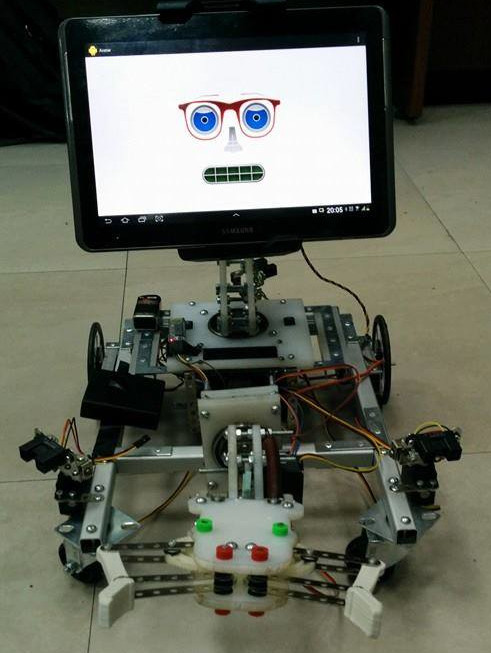
\includegraphics[width = 0.4\textwidth]{images/RoboDroid.jpg}
	\caption{Asistente robótico ``Robodroid'' para terapia de lenguaje e inclusión educativa de niños y niñas con discapacidad \cite{robles2015speltra}.}
	\label{Fig:Robodroid}
\end{figure}

Para interactuar con el asistente robótico, el niño se coloca un guante de color rojo y realiza uno de los seis gestos que se indican en la Figura \ref{Fig:RobodroidGestos}:

\begin{figure}[th!]
	\centering
	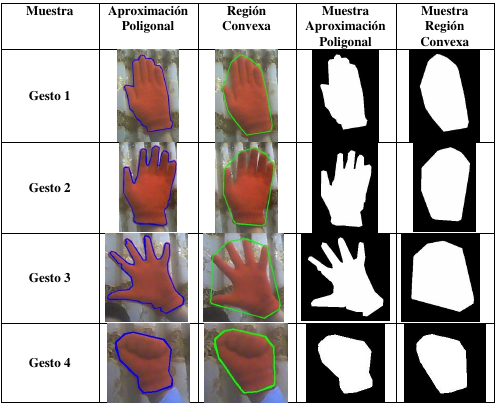
\includegraphics[width = 0.6\textwidth]{images/RobodroidGestos.png}
	\caption{Gestos que permiten controlar e interactuar a los niños con el asistente robótico ``Robodroid'' \cite{ochoa2014diseno}.}
	\label{Fig:RobodroidGestos}
\end{figure}

Cada gesto se puede asignar a una acción específica, por ejemplo, el gesto ``Puño cerrado'' se puede emplear para que los niños seleccionen un color, confirmen una acción, etc.

El proceso para realizar el reconocimiento de los gestos emplea técnicas de visión artificial. Como se puede apreciar en la Figura \ref{Fig:RobodroidProcesoVision}, se llevan a cabo 5 etapas para realizar el reconocimiento de los gestos realizados con el guante. Estas etapas consisten en eliminación de ruido, detección de bordes, realce de contraste, extracción de momentos de Hu, cálculo de la distancia Euclídea e identificación del gesto.

\begin{figure}[th!]
	\centering
	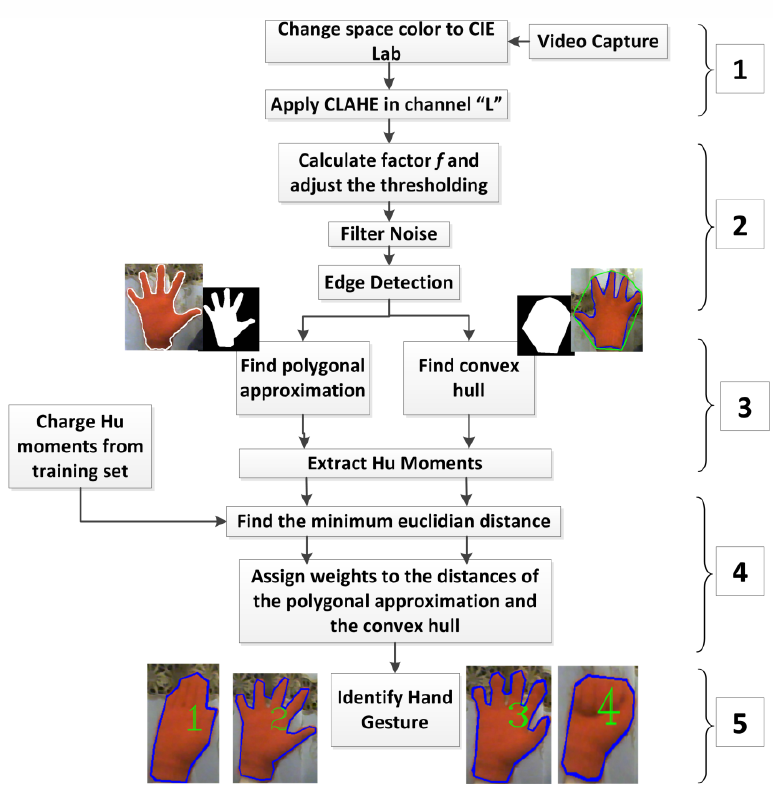
\includegraphics[width = 0.6\textwidth]{images/RobodroidProcesoVision.png}
	\caption{Niños y niñas de la Fundación ``Jesús para los niños''  (Ciudad de Cañar), interactuando con el asistente robótico ``Robodroid'' \cite{ochoa2014diseno}.}
	\label{Fig:RobodroidProcesoVision}
\end{figure}

Por otra parte, en la Figura \ref{Fig:RobodroidTerapia} se puede apreciar a niños de la Fundación ``Jesús para los  niños'' jugando e interactuando con el robot. Luego de realizar varias pruebas, se pudo constatar que los niños tenían mejor predisposición para realizar las terapias y se sentían más motivados por llevar adelante las diferentes actividades.

\begin{figure}[th!]
	\centering
	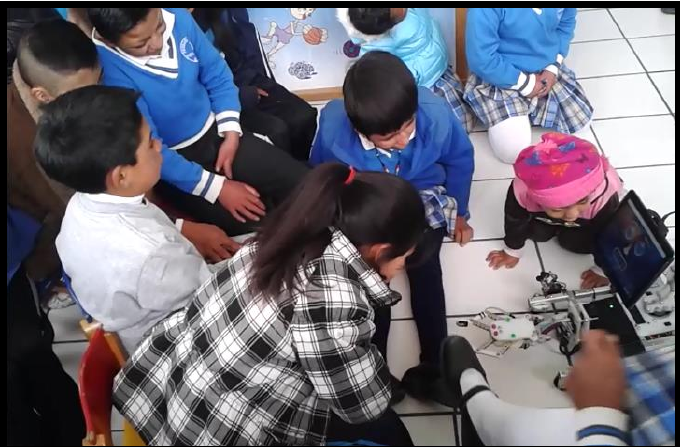
\includegraphics[width = 0.4\textwidth]{images/Robodroid1.png}
	\caption{Niños y niñas de la Fundación ``Jesús para los niños''  (Ciudad de Cañar), interactuando con el asistente robótico ``Robodroid'' \cite{ochoa2014diseno}.}
	\label{Fig:RobodroidTerapia}
\end{figure}


\subsection{Aplicación para reconocimiento de billetes para personas no videntes (2011)}

Las personas no videntes deben afrontar fuertes dificultades para llevar diversas actividades de su vida diaria. Una de ellas, quizá la más compleja, guarda relación con su movilidad.

Generalmente cuando persona no vidente debe desplazarse o adquirir productos, tiene mucha dificultad en determinar la denominación de los billetes con los que realizará el pago. Por ello, en el año 2011, en el GI-IATa se desarrolló un trabajo de titulación que empleó técnicas de visión artificial como \href{https://opencv-python-tutroals.readthedocs.io/en/latest/py_tutorials/py_feature2d/py_sift_intro/py_sift_intro.html}{SIFT} (Scale-Invariant Feature Transform), \href{https://docs.opencv.org/3.0-beta/doc/py_tutorials/py_feature2d/py_surf_intro/py_surf_intro.html}{SURF} (Speeded-Up Robust Features) y \href{https://github.com/opencv/opencv/blob/master/samples/python/asift.py}{A-SIFT} (Affine SIFT) para brindar una herramienta de reconocimiento de billetes a personas no videntes \cite{plaza2011estudio}.

Como se puede apreciar en la Figura \ref{Fig:ReconocimientoBilletes}, la aplicación se desarrolló para dispositivos móviles IPhone\textregistered empleando el lenguaje de programación \href{https://developer.apple.com/library/archive/documentation/Cocoa/Conceptual/ProgrammingWithObjectiveC/Introduction/Introduction.html}{Objective-C} \cite{plaza2011estudio}.

\begin{figure}[th!]
	\centering
	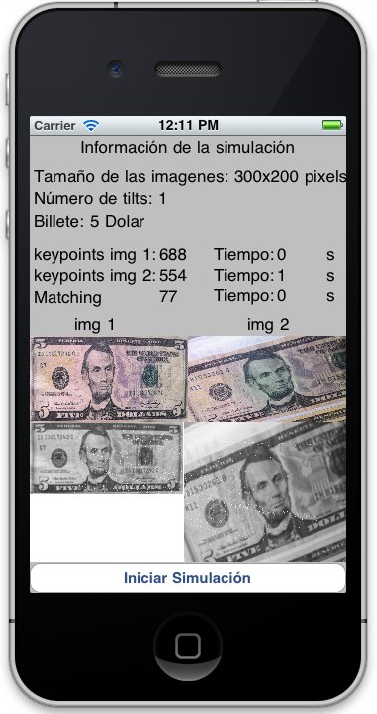
\includegraphics[width = 0.4\textwidth]{images/ReconocimientoBilletesEjemplo.png}
	\caption{Captura de pantalla de la aplicación para reconocimiento de billetes (dólares) para personas no videntes \cite{plaza2011estudio}.}
	\label{Fig:ReconocimientoBilletes}
\end{figure}


Para comunicarse con la persona no vidente la aplicación empleaba la herramienta de Texto a Voz.


\subsection{Aplicación para para terapia de lenguaje y reconocimiento de pictogramas}




\cite{yacchirema2018fall}



\section{Enunciado}

Deberá desarrollar una solución basada en visión artificial que emplee cualquiera de las técnicas vistas durante el taller. Para ello, debe tomar en cuenta las siguientes especificaciones:

\begin{itemize}
	\item El proyecto 
\end{itemize}

\section{Fecha de entrega}



\section{Enlace para la entrega del proyecto}


Instructor: Damodar Rajbhandari, B.Sc. Physics 4th year\\
\hspace*{0.43cm} Registration fee: Free\\
\hspace*{0.43cm} Date: July 18, Tuesday\\
\hspace*{0.43cm}  Time: 11:00 am - 1:00 pm\\
\hspace*{0.43cm} Venue: Loyola Conference Room, St. Xavier's College\\




\vspace{2.8cm}

\begin{center}

\begin{minipage}{0.2\textwidth}
\begin{flushleft}
\rule{3.3cm}{0.4pt} \\[0.5cm]
\textbf{Instructor}\\
\textbf{UPS Sede Cuenca}
V. Robles-Bykbaev
\end{flushleft}
\end{minipage}

\iffalse
~
\begin{minipage}{0.2\textwidth}
\begin{flushleft}
\rule{3.3cm}{0.4pt} \\[0.5cm]
\textbf{HOD of Physics}\\
\textbf{St. Xavier's College}\\
Mr. Drabindra Pandit
\end{flushleft}
\end{minipage}
~
\begin{minipage}{0.21\textwidth}
\begin{flushleft}
\rule{3.4cm}{0.4pt} \\[0.5cm]
\textbf{Moderator}\\
\textbf{SXPC- Nepal}\\
Mr. Basu Dev Ghimire
\end{flushleft}
\end{minipage}
~
\begin{minipage}{0.2\textwidth}
\begin{flushleft}
\rule{3cm}{0.4pt} \\[0.5cm]
\textbf{President}\\
\textbf{SXPC- Nepal}\\
Mr. Binod Bhattarai
\end{flushleft}
\end{minipage}
\fi

\end{center}


\bibliography{Bibliography}
\bibliographystyle{plain}


\end{document}


